%\documentclass[11pt,a4paper,runningheads]{llncs}
\documentclass[11pt,a4paper]{article}
%encoding
%--------------------------------------
\usepackage[T1]{fontenc}
\usepackage[utf8]{inputenc}
%--------------------------------------

%Portuguese-specific commands
%--------------------------------------
\usepackage[portuguese]{babel}
%--------------------------------------

%Hyphenation rules
%--------------------------------------
\usepackage{hyphenat}
\hyphenation{mate-mática recu-perar}
%--------------------------------------

\usepackage{graphicx}
\usepackage{comment}
\usepackage{pgfplots}
\usepackage{amsmath,amssymb,amsfonts}
\usepackage{algorithmic}
\usepackage{graphicx}
\usepackage{textcomp}
\usepackage{xcolor}
\usepackage{adjustbox}
\usepackage{float}
\usepackage[colorlinks=true,urlcolor=blue,linkcolor=black]{hyperref}
\usepackage[scaled]{uarial}
\renewcommand*\familydefault{\sfdefault} %% Only if the base font of the document is to be sans serif


\begin{document}

\title{Fase 3 - Requisitos, Casos de Uso e Arquitetura}
\author{Pedro Carrega, nº49480 \and
Vasco Ferreira, nº49470 \and Ye Yang, nº 49521
}

%\institute{Departamento de Informática da Faculdade de Ciências da Universidade de Lisboa
%\email{\{fc49480,fc49470,fc49521\}@alunos.fc.ul.pt}}

\maketitle

%\renewcommand*\contentsname{Indíce}
\tableofcontents

\section{Motivação para Dataset e Serviços}

O dataset ecommerce foi escolhido pelo grupo devido ao grande número de eventos gerados e consequente informação produzida durante a utilização de uma loja de ecommerce. Informação esta que pode ser utilizada de diversas formas através de um grande número de variados serviços. Essa mesma informação poderá ser utilizada em vários contextos, sendo que escolhemos os seguintes 5 serviços que demonstram diferentes tipos de informação sobre o dataset:

\begin{itemize}
  \item api/products/listCategories: Fornece todas as diferentes categorias presentes nos dados
  \item api/products/popularBrands: Fornece a contagem de eventos associados a cada marca
  \item api/products/salesByBrand: Lista o numero de vendas de cada marca
  \item api/products/salePrice: Calcula o valor médio de venda de uma determinada marca
  \item api/events/ratio: Apresenta a distribuição relativa de cada tipo de evento, havendo os possíveis valores: view, cart e purchase
\end{itemize}

Os serviços foram escolhidos de forma a que consigam fazer diferentes tipos de operações sobre os dados, desde serviços mais específicos e por isso com menos carga na base de dados, a serviços mais abrangentes e consequente aumento de carga. Foram também escolhidos pois todos os serviços fornecem dados úteis para serem explorados no contexto de lojas de ecommerce.

\section{Diagrama de Casos de Uso}
\begin{figure}[H]
  \centering
    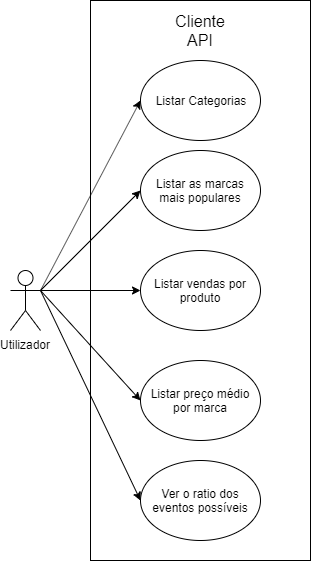
\includegraphics[scale=0.42]{Use_Cases.png}
  \caption{Diagrama de casos de uso}
\end{figure}

\section{Requisitos}

\begin{table}[H]
	\begin{center}
		\begin{tabular}{|p{3.5cm}|p{9.5cm}|}
		\hline
			\textbf{Requisitos\newline Não Funcionais} & \textbf{Descrição}\\ \hline
			Portabilidade & Implementação de servidor em NodeJS e cliente em HTML de modo a facilitar o processo de mudança de plataforma do serviço \\ \hline
			Legibilidade & A separação clara entre as camadas de apresentação, lógica de negócio e acesso à base de dados irá tornar o fluxo do sistema mais legível para os desenvolvedores \\ \hline
			Estabilidade & A distribuição do sistema por diversas máquinas virtuais, que poderão estar distribuídas por diferentes fornecedores cloud e em diferentes Data Centers permitem obter um sistema estável \\ \hline
			Elasticidade & O sistema deverá ser capaz de se adaptar à carga de trabalho através do provisionamento e desprovisionamento dos recursos de forma autónoma. Idealmente, de forma que em qualquer ponto do tempo, o sistema apenas utilize o número de máquinas necessárias de forma a corresponder à carga atual \\ \hline
			Escalabilidade & Capacidade do sistema lidar com o crescimento de carga de trabalho. Pode-se associar à capacidade de elasticidade do sistema \\ \hline
			Confiabilidade & Visto o sistema estar implementado na núvem, conseguimos garantir alta confiabilidade nos sistema, pois se um servidor no datacenter falhar, conseguimos facilmente migrar a VM para outro servidor funcional \\ \hline
	\end{tabular}
	\label{tab1}
	\end{center}
	\caption{Requisitos Não Funcionais}
\end{table}

\begin{table}[H]
	\begin{center}
		\begin{tabular}{|p{3.8cm}|p{8.2cm}|}
		\hline
			\textbf{Requisitos\newline Funcionais} & \textbf{Descrição}\\ \hline
			Listar\newline Categorias Disponíveis & Serviço que fornece aos clientes todas as categorias \\ \hline
			Visualizar\newline Popularidade das\newline Marcas & Serviço que fornece cada marca associada com a sua popularidade\\ \hline
			Visualizar\newline Número de Vendas\newline Individuais & Fornece o numero total de vendas de cada marca\\ \hline
			Visualizar\newline Preço Médio de Venda & Fornece o preço médio dos produtos vendidos de uma determinada marca \\ \hline
			Visualizar\newline Rácio de Tipo\newline de Eventos & Fornece a percentagem de cada tipo de evento \\ \hline
	\end{tabular}
	\label{tab2}
	\end{center}
	\caption{Requisitos Funcionais}
\end{table}

\section{Arquitetura da aplicação}
\begin{figure}[H]
  \centering
  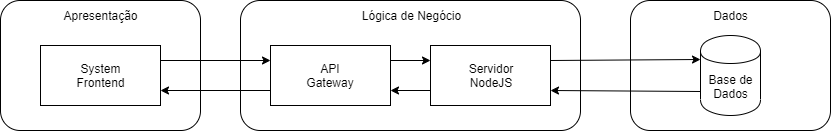
\includegraphics[scale=0.4]{App_arc.png}
  \caption{Arquitetura da aplicação}
\end{figure}

Após a definição da API na fase anterior, foi implementado de raiz um servidor em NodeJS que segue a API definida.


\subsection{Load Balancer}
Foi implementado um Load Balancer que distribui os pedidos HTTP recebidos dos clientes browser e que reencaminha para os respetivos serviços.


\subsection{Servidor NodeJS}
O servidor irá receber os pedidos a partir do Load Balancer, e processá-los de acordo com a funcionalidade pretendida. A lógica de negócio é aqui tratada, realizando as queries necessárias para a base de dados. Ao receber os dados, processa-os de acordo com a funcionalidade, e encaminha o resultado para o Load Balancer.
%\newline %removam isto se nao gostarem do espaço k adiciona

\subsection{Base de dados}
A base de dados irá conter o conteúdo dos ficheiros .csv do nosso dataset, que são acedidos pelo servidor de modo a poder efetuar as leituras necessárias para produzir uma resposta para o cliente. 
%\newpage

\section{Arquitetura técnica}
%Digam-me o que acham

%Não sei o que dizer da Portabilidade
Para garantir os requisitos não funcionais mencionados a cima devemos ter em atenção os serviços da cloud escolhidos, pois proporcionam vários aspetos fundamentais dos requisitos.
\newline

A utilização dos serviços disponibilizados pela AWS permite cumprir alguns dos requisitos não funcionais mencionados, nomeadamente a Escalabilidade e a Elasticidade. Já o Load Balancer implementado com o Ingress permite que este serviço da cloud trate automaticamente da separação dos diferentes tipos de pedidos HTTP recebidos para os respetivos serviços. A base de dados utilizada consiste uma imagem docker baseada na imagem mongo que como o nome sugere é uma imagem de MongoDB. Foi escolhida esta alternativa de forma a não estar dependente dos serviços de Bases de Dados de um fornecedor específico, sendo que com esta opção a imagem pode ser implementada numa instância em qualquer fornecedor cloud. Quanto à escalabilidade a imagem poderia ser replicada por diversas réplicas de forma a distribuir os pedidos feitos pelas diferentes réplicas.  %NOT TOTALY SURE,devemos por isto?
\newline

A Confiabilidade do sistema também é melhorada com a instalação em serviços na cloud, visto estas terem deteções automáticas de falhas de servidores, possibilitando a migração do sistema virtualizado para outro servidor funcional.
\newline

A Estabilidade é garantida nas várias ferramentas usadas na instalação do sistema. O Load Balancer como referido anteriormente faz a distribuição dos pedidos HTTP para os respetivos serviços, sendo que o Kubernetes atribui um DNS igual para todas as réplicas do serviço de maneira a que o Load Balancer apenas reencaminhe para o respetivo DNS, sendo o Kubernetes a distribuir a carga pelas respetivas réplicas do serviço. Isto permite que o sistema escale com facilidade já que aumentar o número de réplicas de um micro-serviço em Kubernetes é um processo rápido e sem necessitar de qualquer alteração no Load Balancer.
\newline

Já a Estabilidade é garantida devido a ter a Lógica de negócio distribuída por várias máquinas virtuais que cumprem a função de servidores.
\newline


A utilização do Docker permite-nos facilmente fazer deploy de um serviço, em qualquer máquina e em qualquer um fornecedor de cloud. Isto deve-se ao Dockerfile garantir a instalação de todas as dependências do serviço, variando conforme a linguagem de implementação do mesmo, cumprindo assim o requisito de Portabilidade do sistema.

\section{Implementação}

\subsection{Base de dados}
Uma das maiores dificuldades que tivemos foi a passagem dos dados em formato CSV para uma tabela na DynamoDB. Começamos primeiro com a criação de scripts em Python, com a utilização de bibliotecas disponibilizadas pela AWS. Isto mostrou-se não fazível devido às limitações do tamanho do heap e da memória consumida, visto o ficheiro CSV ser de grandes dimensões.

Passamos para a implementação do mesmo script mas através do AWS Lambda mas deparamo-nos com o mesmo problema, sem sucesso na escrita para a DynamoDB.

Finalmente utilizamos a ferramenta do Data Pipeline, que por sua vez originou vários novos obstáculos:
\begin{enumerate}
	\item Deparamo-nos com vários erros na passagem do CSV para a DynamoDB. Estes erros originaram do facto da DynamoDB ter um formato específico de JSON que contém não só o nome de cada coluna, como o tipo da coluna. Esta informação não se encontrava explicitamente documentada, logo para obter a estrutura tivemos que escrever uma linha manualmente numa tabela criada, exportar usando o Data Pipeline para um bucket S3 e daí conseguimos observar a estrutura. De seguida criamos um parser que percorria o dataset, eliminando espaços vazios que não são aceitadas pela DynamoDB, tornando cada linha no formato JSON que a DynamoDB conseguisse interpretar.
	
	\item No início da utilização do Data Pipeline, o tempo de escrita para a tabela aparentava ser muito elevado, rondando os 15 minutos para um ficheiro de 8MB. Isto deve-se ao facto das tabelas da DynamoDB terem um controlo da taxa de transferência, que caso for demasiado elevada, consumia para além do que o free tier da AWS fornecia, consumindo recursos monetários em elevadas quantidades na nossa experiência.
	
	\item Na implementação das queries para a DynamoDB, reparamos numa limitação dos resultados obtidos com o despoletar de uma query. Isto deve-se ao facto da DynamoDB limitar os resultados de cada query a "páginas" de 1MB, sendo que uma página é um conjuntos das entradas filtradas pela query. Tivemos então que lidar com a paginação, que provou ser pouco eficiente, baseando-se na utilização da última entrada da página anterior, e despolentando uma nova query a partir dessa entrada, logo necessitando de \textit{TAMANHO\_DATASET}/1MB queries.
	
	\item As queries da DynamoDB são de 2 tipos: \textbf{Scan} e \textbf{Query}. Inicialmente usamos Scans para alguns serviços disponibilizados, porém, estes eram muito ineficientes em comparação com as queries dado que necessitavam de percorrer a tabela inteira. Recriamos então a tabela, de modo a fornecer uma Primary Key comum a todas as entradas e com uma coluna \textbf{event\_id} que era denominada como Sorting Key, distinguindo todas as entradas. Isto possibilitou a utilização de queries da DynamoDB que aumentou o desempenho para certos serviços. 
	
	\item Porém, existiam outros serviços (como o caso do \textit{/api/events/ratio}) que necessitavam de percorrer a base de dados na sua totalidade para mostrar as estatísticas pretendidas, pelo que não se verificou um aumento de desempenho significante entre a utilização de Queries ou Scans. Estas queries demoravam em média 10 a 15 minutos por cada pedido realizado, não sendo um tempo de execução aceitável.
	
	\item Foi concluído que a DynamoDB não era uma base de dados adequada para a realização de análise de dados. Daí, mudamos a implementação para uma imagem Docker de Mongo.
\end{enumerate}

Ao apercebemo-nos de que DynamoDB não seria a melhor escolha para a base de dados tendo em conta os serviços definidos e o dataset usado, decidimos mudar para uma base de dados Mongo em que manteríamos uma base de dados NoSQL, já que nos permite uma escalabilidade horizontal que se adequa aos serviços fornecidos.
Verificamos que utilizar o serviço fornecido pelo MongoDB Atlas tinha custos dos quais não poderíamos suportar, optámos então por utilizar a imagem Mongo disponibilizada online. Mas isto não seria suficiente, pois queríamos que o processo fosse simples, tal como montar qualquer outro container, mas para isso queríamos que a imagem contivesse os dados do dataset para que ao ser montada, começaria a auto popular-se de acordo com o CSV importado. Para conseguir obter esta simplicidade, recorremos a um Dockerfile que usasse como imagem base a imagem de Mongo mas que tal como necessitaríamos, acrescentasse um novo conjunto de operações. Portanto adicionamos a funcionalidade de, ao dar build, copiar o ficheiro CSV com os dados do dataset para a imagem a construir, de seguida necessitámos de definir um shell script que fosse executado depois de correr a imagem. Para isso definimos um simples script que trataria de executar a base de dados e consequentemente importasse os dados contidos no ficheiro CSV presente na imagem. Ao definir o seguinte script, o mesmo foi acrescentado como entrypoint no Dockerfile para que fosse executado assim que a imagem fosse corrida. Foi também acrescentada a cópia do script para o container tal como foi feito anteriormente com o ficheiro CSV.
Depois de definir toda esta estrutura construimos a imagem e fizemos push para um repositório da AWS para que ficasse acessível. Assim conseguimos obter uma imagem de uma Base de Dados Mongo que é facilmente montada em qualquer máquina devido à utilização do Docker. Bastando puxar a imagem do repositório e correr como qualquer outra imagem.

Depois de toda esta preparação tivemos de converter todas as nossas queries definidas para cada serviço, a principal vantagem nesta nova base de dados seria o uso do distinct, sendo que o Mongo apesar de tal como a Dynamo  ser também NoSQL, permite uma mais fácil implementação de queries mais complexas, sendo que os serviços fornecidos iriam tirar bastante proveito das melhorias. Deparamo-nos então com um problema semelhante à paginação da Dynamo mas agora em Mongo, neste caso uma query ao devolver demasiados resultados devolve um cursor que tem de ser iterado para devolver passo a passo, todos os dados resultantes da query. Inicialmente deparamo-nos com alguma dificuldade na utilização do cursor já que não conseguimos encontrar uma documentação muito clara e completa. Depois de alguma insistência da parte do grupo, conseguimos através de várias tentativas, compreender como iterar sobre um cursor e assim tirar proveito das queries. Após ultrapassada esta dificuldade, todas as queries foram facilmente implementadas, sendo que foi usada principalmente a operação de agregate que permite uma maior complexidade das queries permitindo assim filtrar ao máximo a resposta da Base de dados, reduzindo assim a latência de resposta, já que era esse o grande problema das queries da DynamoDB que devolviam demasiadas entradas forçando assim a existir muitas trocas de dados com consequente acréscimos de latência em cada resposta.
Com esta implementação das queries de forma mais detalhada, conseguimos assim um aumento de performance muito significativo relativamente à Dynamo, provando que a mudança de Base de dados apesar de ter custado algum tempo para efetuar depois de termos feito toda a implementação para Dynamo, foi a escolha certa a fazer tornando assim o nosso serviço mais eficiente, passando a ter respostas da parte da Base de dados na ordem de poucos segundos ao contrário dos anterior minutos necessários para devolver uma resposta.

\subsection{Web Server}
O Web Server foi inicialmente implementado em NodeJS com um router Koa. Porém a documentação relativa ao router era escassa em comparação a outras alternativas, razão pela qual mudamos para um router Express que se encontrava com melhor documentação.

As queries para a base de dados na DynamoDB foram implementadas em NodeJS, onde foi necessário tratar da paginação. A documentação relativa à paginação das queries encontrava-se disponível sendo a implementação relativamente simples, excluindo as tentativas de melhorar o desempenho.

Mudando a implementação da base de dados para uma de MongoDB, deparamo-nos com pequenos problemas de implementação das queries, mas que foram eventualmente resolvidos, observando-se um aumento de desempenho a várias ordens de magnitude em comparação com a implementação na DynamoDB (queries que demoravam 10-15 minutos na Dynamo não excediam os 20 segundos no mongo).

\subsection{Load Balancer}
Para o balanceamento da carga no deployment em Kubernetes, utilizamos um controlador de Ingress, o NGINX. Este controlador encaminha os vários pedidos para os serviços correspondentes. No nosso caso concretamente, os pedidos com o URL \textit{/api/events*} e \textit{/api/products*} são encaminhados para os seus respetivos serviços que estão deployed nas Kubernetes. Os serviços por sua vez fazem o balanceamento de carga automaticamente pelos vários pods por nós lançados que contém a implementação do Web Server.

Na implementação do Ingress controller deparamo-nos com problemas no deployment do Ingress em si, pois este não mostrava o endereço necessário para realizar o load balancing, não conseguimos antes da primeira entrega encontrar o problema no nosso deployment, pelo que tivemos que fazer expose dos 2 serviços individualmente para ter um sistema que responda a queries.

Já na segunda entrega fizemos uma nova implementação do controlador Ingress, desta vez dando as permissões necessárias e acrescentado os dados corretos no ficheiros YAML relacionados com o Ingress, resultand num deployment correto do load balancer.
\section{Lançamento em Kubernetes}
O scripts de deployment do sistema foram separados em 4 devido à necessidade dos clusters e node groups estarem ativos, antes de proceder aos próximos passos. Existe também uma secção de edição de ficheiro manual, o que fez a quebra entre o terceiro e o quarto script.

Antes da execução dos scripts é necessário verificar a existência dos seguintes repositórios, roles e policies e caso existam, precisam de ser \textbf{eliminados}:
\begin{enumerate}
	\item Repositórios com nomes \textit{products} e \textit{events}
	\item AWS Role com nome eksServiceRole
	\item AWS Policy com nome ALBIngressControllerIAMPolicyEcommerce
\end{enumerate}

Para a execução dos scripts são necessárias as seguintes ferramentas:
\begin{itemize}
	\item AWS CLI
	\item eksctl
	\item kubectl
\end{itemize}

A região a escolher para o lançamento poderá ser qualquer um, porém recomendamos a região eu-west-1. Esta região terá de ser a mesma nos argumentos de todos os scripts que requeiram a mesma.

Com a utilização do Ingress, reparamos que existe a possibilidade deste poder usar VPCs antigas, para prevenir que tal ocorra, sugerimos apagar Target Groups que não estejam a ser utilizados.

\subsection{deploy1.sh}
O primeiro script de deployment recebe 3 argumentos na seguinte ordem:
\begin{enumerate}
	\item A região onde a Stack e o Cluster vão ser lançados (ex.: \textbf{eu-west-1})
	\item O nome da Stack que terá de ser único (nenhuma outra Stack na CloudFormation da conta pessoal poderá ter o mesmo nome) para o script funcionar corretamente (ex.: \textbf{ecommerce-stack})
	\item O nome do Cluster que também terá de ser único (ex.: \textbf{ecommerce-cluster})
	\item Exemplo de execução: \textit{./deploy1.sh eu-west-1 e-stack e-cluster}
\end{enumerate}

A criação da stack e do cluster irá demorar cerca de 10 a 20 minutos até ficarem ativos, após o qual poderemos proceder à execução do segundo script. O estado do script pode ser verificado com o seguinte comando:
\begin{itemize}
	\item \textit{aws eks describe-cluster \texttt{-{}-}name CLUSTER\_NAME} , mudando CLUSTER\_NAME para o nome do cluster dado nos argumentos
\end{itemize}
A execução do segundo script só deve ser feita quando o estado do cluster estiver em \textbf{ACTIVE}.

\subsection{deploy2.sh}
O segundo script recebe os mesmos argumentos que o primeiro, todos na mesma ordem. Neste script vão ser criados os node groups e o pull das imagens dos serviços.

Para realizar o pull, irá ser pedido para inserir os credenciais IAM que dão acesso aos repositórios por nós criados. Estes credenciais encontram-se no ficheiro \textbf{credenciais.txt} juntamente com a região onde os repositórios se encontram.

No fim da execução do script, é necessário verificar o estado dos node groups antes de proceder ao próximo script. O estado pode ser verificado com o seguinte comando: 
\begin{itemize}
	\item \textit{aws eks describe-nodegroup \texttt{-{}-}cluster-name CLUSTER\_NAME \texttt{-{}-} nodegroup STACK\_NAME} , mudando CLUSTER\_NAME e STACK\_NAME para os respetivos nomes dados nos argumentos
\end{itemize}
No final irá ser pedido para introduzir os credenciais de IAM para a conta de AWS pessoal de modo a poder criar os repositórios e fazer push das imagens no script seguinte.
Após o estado do node group passar para \textbf{ACTIVE} podemos proceder À execução do terceiro script.

\subsection{deploy3.sh}
O terceiro script recebe 2 argumentos na seguinte ordem:
\begin{itemize}
	\item A região que deverá ser idêntica às inseridas nos scripts anteriores
	\item O nome do cluster que também deverá ser o mesmo
\end{itemize}
Para a correto funcionamento deste script, salienta-se a necessidade de apagar os repositórios, roles e policies anteriormente referidos.

Após a criação dos repositórios e o push das imagens para os mesmos, será pedido para mudar os credenciais IAM para os que se encontram no ficheiro \textbf{credenciais\_mongo.txt} para realizar o pull da imagem da base de dados.

Depois de realizar o pull irá ser pedido para mudar os credenciais de novo para a conta pessoal de AWS para a criação do repositório da base de dados e o push da imagem.

\subsection{deploy4.sh}
Antes da execução do 4 ficheiro de deployment, as seguintes mudanças terão de ser realizadas nos ficheiros \textbf{ingress/ingress-rbac.yaml} e \textbf{ingress/alb-ingress-controller.yaml}.

\subsubsection{ingress/ingress-rbac.yaml}
Neste ficheiro é necessário inserir manualmente os dados relativos ao role criado no ficheiro na seguinte linha:
\begin{itemize}
	\item \textbf{eks.amazonaws.com/role-arn:}
\end{itemize}
Para aceder ao valor do ARN do role criado, basta inserir na linha de comandos as seguintes instruções:
\begin{itemize}
	\item \textbf{aws iam get-role \texttt{-{}-}role-name eksServiceRole}
\end{itemize}

\subsubsection{ingress/alb-ingress-controller.yaml}
Neste ficheiro é necessário inserir a informação relativa ao cluster criado para que o Ingress utilize os recursos corretos. Para tal é necessário alterar no ficheiro, na linha: 
\begin{itemize}
	\item \textbf{- \texttt{-{}-}cluster-name=CLUSTER\_NAME}
\end{itemize}
alterando \textbf{CLUSTER\_NAME} pelo nome do cluster dado nos argumentos dos scripts anteriores.

Na linha:
\begin{itemize}
	\item \textbf{- \texttt{-{}-}aws-vpc-id=VPC\_ID}
\end{itemize}
alterar \textbf{VPC\_ID} pelo ID do VPC gerado na criação da Stack. Este ID pode ser verificado correndo o script \textbf{get-vpc-id.sh} com os seguintes parametros de entrada:
\begin{itemize}
	\item A região onde a Stack foi criada
	\item O nome da stack dado na criação
\end{itemize}
Exemplo de execução: \textbf{./get-vpc-id.sh eu-west-1 stack}

Após a execução destes 2 passos, executa-se o quarto e último script, \textbf{deploy4.sh} sem parâmetros de entrada.

\subsection{Acesso aos serviços}
Após a aplicação dos ficheiros yaml do Ingress, é possível aceder ao sistema executando o comando:
\begin{itemize}
	\item \textbf{kubectl get ingress}
\end{itemize}
Deste comando retira-se o endereço que se encontra em \textit{Address} e adiciona-se os paths para os serviços disponibilizados (ex.: <address>/api/products/ listCategories).

\subsection{Desconstrução do deployment}
Para remover a montagem do sistema, seguem-se os seguintes passos:
\begin{enumerate}
	\item Na consola de \href{https://eu-west-1.console.aws.amazon.com/eks/home?region=eu-west-1#/clusters}{EKS}, dependendo da região escolhida, selecionar o cluster e apagar o node group correspondente. Após dos node groups terem sido eliminados, proceder com a eliminação do cluster.
	\item Na consola de \href{https://eu-west-1.console.aws.amazon.com/ec2/v2/home?region=eu-west-1#LoadBalancers}{EC2}, eliminar os load balancers criados. Na mesma consola navegar para os target groups e apagar aqueles que estejam relacionados com o VPC criado.
	\item Na consola de \href{https://eu-west-1.console.aws.amazon.com/vpc/home?region=eu-west-1#NatGateways}{VPC}, eliminar as NATs criadas. Após a eliminação, navegar para a secção dos VPCs e eliminar as VPCs correspondentes que contém o nome dado à stack.
	\item Na consola de \href{https://console.aws.amazon.com/ecr/repositories?region=us-east-1}{ECR}, eliminar os seguintes repositórios: \textit{database}, \textit{events} e \textit{products}.
	\item Na consola de \href{https://console.aws.amazon.com/iam/home?#/policies}{IAM Policies}, eliminar a policy com o seguinte nome: \textbf{ALBIngressControllerIAMPolicyEcommerce}. Após a eliminação, navegar para a secção dos Roles, e apagar o role com o seguinte nome: \textbf{eksServiceRole}.
	\item Na consola de \href{https://eu-west-1.console.aws.amazon.com/cloudformation/home?region=eu-west-1#/stacks}{CloudFormation}, eliminar a stack criada com o nome dado nos scripts anteriores.
\end{enumerate}

\section{Cenários de Validação}

\begin{itemize}
	\item Listar Categorias:
	\begin{enumerate}
		\item Inserir o url mencionado posteriormente.
		\item Após alguns segundos irá aparecer no ecrã o resultado.
	\end{enumerate}
	\item Listar a popularidade das marcas:
	\begin{enumerate}
		\item Inserir o url mencionado posteriormente.
		\item Após alguns segundos irá aparecer no ecrã o resultado.
	\end{enumerate}
	\item Listar vendas de cada marca:
	\begin{enumerate}
		\item Inserir o url mencionado posteriormente.
		\item Após alguns segundos irá aparecer no ecrã o resultado.
	\end{enumerate}
	\item Listar o preço médio de uma marca:
	\begin{enumerate}
		\item Inserir o url mencionado posteriormente adicionado "/<Marca>", aonde <Marca> representa a marca que o utilizador quer analisar.
		\item Após alguns segundos irá aparecer no ecrã o resultado.
	\end{enumerate}
	\item Ver o ratio dos eventos possíveis:
	\begin{enumerate}
		\item Inserir o url mencionado posteriormente.
		\item Após alguns segundos irá aparecer no ecrã o resultado.
	\end{enumerate}
	\item Portabilidade:
	\begin{enumerate}
		\item 
	\end{enumerate}
	\item Legibilidade:
	\begin{enumerate}
		\item 
	\end{enumerate}
	\item Estabilidade:
	\begin{enumerate}
		\item 
	\end{enumerate}
	\item Elasticidade:
	\begin{enumerate}
		\item Verfique o numero de worker nodes ativos
		\item 
	\end{enumerate}
	\item Escalabilidade:
	\begin{enumerate}
		\item 
	\end{enumerate}
	\item Confiabilidade:
	\begin{enumerate}
		\item 
	\end{enumerate}
\end{itemize}

\section{Conclusão e Discussão}
Durante o desenvolvimento do projeto foram encontrados bastantes obstáculos, seja na implementação dos serviços, na escolha e consequente aplicação da base de dados ou na automatização dos scripts de implementação dos serviços desenvolvidos. Todos estes problemas resultaram em muitas horas de trabalho extra por parte do grupo, mas serviram também de aprendizagem, seja em como trabalhar com fornecedores de serviços na nuvem, ou o desenvolvimento de scripts de automatização de deployment. Apesar de todos os problemas, o grupo foi capaz de os solucionar de forma eficiente como mencionados na secção da Arquitetura técnica.

\end{document}